
\chapter{Spickzettel}

Autor: Gerhard Gossen

Dieser \glqq Spickzettel\grqq{} enthält grundlegende Definitionen und
Schreibweisen, die du im Studium und im Vorkurs brauchst. Wir werden den Inhalt im Kurs
meist voraussetzen.

\section{Zahlenbereiche}
{
\begin{tabular}{lp{18em}p{7em}}
 \textbf{Zeichen} & \textbf{Beschreibung} & \textbf{Beispiele}\\
\hline 
$\mathbb{N}$ & Natürliche Zahlen: Positive ganze Zahlen Die $0$ ist
 meistens  nur enthalten, wenn die Bezeichnung $\mathbb{N}_0$ verwendet
  wird
 & $1$; $2$;
$3$; $454647$; $8892349823$\\
$\mathbb{Z}$ & Ganze Zahlen: Alle positiven und negativen ganzen Zahlen (engl.
ganze Zahl: \emph{integer}) &
$-2$; $-1$; 0; 1; 2; 42; $-645631$; $3469079$ \\
$\mathbb{Q}$ & Rationale Zahlen: Zahlen, die sich als Bruch von zwei ganzen Zahlen darstellen lassen &
$\frac{1}{2}$; $\frac{1}{3}$; $\frac{4}{3}$; $-\frac{6}{23}$; $0.2 (=\frac{1}{5})$  \\
$\mathbb{R}$ & Reelle Zahlen & $1,25; \sqrt{2}; \pi$\\
$\mathbb{C}$ & Komplexe Zahlen (siehe Kap.~\ref{chap:complex}) & $2 + 3i; i;
-6 - 42i$
\end{tabular}
}

\vspace{1em}
Jeder Zahlbereich enthält alle Zahlbereiche darüber:
$\mathbb{N} \subset \mathbb{Z} \subset \mathbb{Q} \subset \mathbb{R} \subset \mathbb{C}$

\section{Mengen}
Mengen können auf verschiedene Arten dargestellt werden. Die beiden 
wichtigsten sind diese:
\begin{itemize}
 \item explizite Auflistung: $M = \{a, b, c, d\}$ enthält die Elemente $a, b, c$ und $d$.
 \item Angabe einer zu erfüllenden Bedingung: $M = \{x \in \mathbb{N}\, |\, 0 < x < 42 \}$ 
    enthält alle natürlichen Zahlen zwischen $0$ und $42$ (ohne diese beiden Zahlen).
\end{itemize}

Seien $A$, $B$ zwei Mengen. Dann sind die folgenden Operationen definiert:

\begin{tabular}{ccc}
 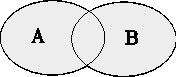
\includegraphics{img/vereinigung.pdf} &
 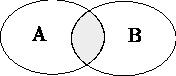
\includegraphics{img/durchschnitt.pdf} &
 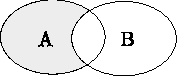
\includegraphics{img/differenz.pdf} \\
 Vereinigung & Durchschnitt & Differenz \\
 $A \cup B$ & $A \cap B$ & $A \setminus B$
\end{tabular}

\vspace{1em}\par

\emph{$a$ ist Element von $A$}: $a\in A$.

Die \emph{leere Menge} ($\emptyset$) ist die Menge, die keine Elemente hat.

Zwei Mengen sind gleich ($A=B$), wenn beide aus den selben Elementen bestehen.

\begin{itemize}
\item Zwei Mengen heißen \emph{disjunkt}, wenn sie keine gemeinsamen Elemente haben:
$A\cap B = \emptyset$.

\item Eine Menge $A$ kann vollständig in einer anderen Menge $B$ enthalten sein: 
$A\subseteq B$ (sprich: \emph{$A$ ist eine Teilmenge von $B$}). Wenn $A\neq B$ 
gilt, ist $A$ eine \emph{echte Untermenge} von $B$ ($A \subset B$).

\item Analog ist definiert: $A$ ist eine (echte) Obermenge von $B$: $A \supseteq B$ 
($A \supset B$).

\item Die \emph{Komplementmenge} $\overline{A}$ der Menge $A$ enthält alle Elemente,
die in $A$ nicht enthalten sind. Wenn $A$ eine Teilmenge einer Trägermenge $X$
ist, dann gilt: $\overline{A} = X\setminus A$

\end{itemize}

\begin{table}
\begin{tabular}{cclp{17em}}
\textbf{klein} & \textbf{groß} & \textbf{Name} & \textbf{übliche Verwendung}\\
\hline
$\alpha$& & Alpha & Winkel\\
$\beta$ & & Beta & Winkel\\
$\gamma$ & $\Gamma$ & Gamma & \\
$\delta$ & $\Delta$ & Delta & $\Delta$: Differenz\\
$\varepsilon$ & & Epsilon & sehr kleine positive Zahl\\
$\eta$ & & Eta\\
$\theta$ & $\Theta$ &  Theta & $\theta$: Winkel in Polarkoordinaten\\
$\lambda$ & &  Lambda & multiplikativer Faktor\\
$\mu$ & & My\\
$\xi$ & & Xi \\
$\pi$ & $\Pi$ & Pi & $\pi = 3,14\dots$, $\Pi$: Multiplikation\\
$\rho$ & & Rho\\
$\sigma$ & $\Sigma$ & Sigma & $\Sigma$: Summe\\
$\tau$ & & Tau \\
$\phi$ & $\Phi$ & Phi & $\phi$: Winkel \\
$\chi$ & & Chi \\
$\psi$ & $\Psi$ & Psi \\
$\omega$ & $\Omega$ & Omega\\
\end{tabular}
\label{tab:griechisch}
\caption{Auswahl von wichtigen griechischen Buchstaben}
\end{table}


\section{Intervalle}
Ein Intervall ist ein zusammenhängender Zahlenbereich, der durch seine beiden
Endpunkte bestimmt ist. Es wird zwischen geschlossenen und
offenen Intervallen unterschieden. Ein \emph{geschlossenes Intervall}
$[a,b]$ enthält $a$ und $b$ (inklusiv), ein \emph{offenes Intervall}
$(a,b)$ enthält $a$ und $b$ nicht mehr (exklusiv).

Es ist möglich, beide Arten zu kombinieren. Es entsteht ein
\emph{halboffenes Intervall}: $[a,b)$ enthält $a$, aber nicht $b$, während
$(a,b\,]$ hingegen $b$, aber nicht $a$ enthält.

\begin{table}[htb]
\begin{tabular}{ll}
\textbf{Symbol} & \textbf{Bedeutung}\\\hline
 $\exists x$    & es existiert (mindestens) ein $x$\\
 $\nexists x$   & es existiert kein  $x$\\
 $\forall x$    & für alle $x$ gilt \dots\\
 $\pm$          & Plus/Minus, z.\,B. $x_{1,2} = \pm 1 \rightarrow x_1 = -1,
x_2 = +1$\\
 $\sum\limits_{i=1}^n a_i$ & $a_1 + a_2 + \dots  + a_n$ \\
 $\prod\limits_{i=1}^n a_i$ & $a_1 \cdot a_2 \cdot\  \cdots\ \cdot a_n$\\
 $\infty$       & Unendlich \\
 $\wedge$       & logisches und\\
 $\vee$         & logisches oder\\
 $\neg$         & logische Negation\\
 $:=$           & ist definiert als\\
 $<,\leq$       & kleiner als, kleiner oder gleich (oft auch: \glqq echt
kleiner, kleiner\grqq)\\
 $>,\geq$       & größer als, größer oder gleich (oft auch: \glqq echt
größer, größer\grqq)\\
 $=, \neq$      & gleich, ungleich\\
\end{tabular}
\label{tab:zeichen}
\caption{Wichtige Sonderzeichen}
\end{table} 


\section{Abkürzungen und Vokabeln}
\begin{description}
 \item[gdw.] Kurz für \glqq genau dann, wenn\grqq. Als Symbol wird auch
$\Leftrightarrow$ verwendet.
 \item[qed] Am Ende eines Beweises. Lateinisch \glqq quod erat
demonstrandum\grqq{} (\glqq was zu zeigen/ beweisen war\grqq). Bedeutung:
Hurra, wir haben den Beweis endlich hinter uns. Gedruckt wird auch
das Zeichen $\square$ verwendet.
 \item[kommutativ] \glqq vertauschbar\grqq. Eine Operation (z.B. $+,\cdot$)
ist kommutativ, wenn man die beiden Operanden vertauschen kann, ohne das
Ergebnis zu ändern. Als Formel ausgedrückt, heißt das: $a\circ b = b\circ a$,
wobei $\circ$ für die Operation steht.
 \item[distributiv] Ausklammern ist erlaubt: $a\cdot(b+c) = a\cdot b + a\cdot
c$
 \item[assoziativ] Die Reihenfolge, in der die Operation durchgeführt wird,
ist beliebig: $a+b+c = (a+b)+c = a+(b+c)$.
 \item[es existiert ein] Es gibt \emph{mindestens} ein Element, das die
Aussage erfüllt.
 \item[es existiert genau ein] Es gibt nur ein einziges Element, das die
Aussage erfüllt.
 \item[notwendige Bedingung] Diese Bedingung ist immer erfüllt, falls eine Aussage gilt. Es gibt aber auch Fälle, in denen die Bedingung erfüllt ist, obwohl die Aussage nicht gilt.
 \item[hinreichende Bedingung] Wenn diese Bedingung erfüllt ist, gilt die Aussage auf jeden Fall. Es gibt aber Fälle, in denen die Aussage gilt, die Bedingung aber nicht erfüllt ist.
 \item[notwendige und hinreichende Bedingung] Immer dann, wenn diese Bedingung erfüllt ist, gilt auch die Aussage (und umgekehrt).
\end{description}

%\pagebreak

%\section{Wichtige griechische Buchstaben}
%Tabelle~\ref{tab:griechisch} enthält eine Auswahl mit Buchstaben, denen du begegnen
%wirst, und ihre übliche Verwendung.

%\section{Komische Zeichen}
%Tabelle~\ref{tab:zeichen} enthält eine Übersicht der wichtigsten mathematischen Zeichen.

